%%%%%%%%%%%%%%%%%%%%%%%%%%%%%%%%%%%%%%%%%
% baposter Portrait Poster
% LaTeX Template
% Version 1.0 (15/5/13)
%
% Created by:
% Brian Amberg (baposter@brian-amberg.de)
%
% This template has been downloaded from:
% http://www.LaTeXTemplates.com
%
% License:
% CC BY-NC-SA 3.0 (http://creativecommons.org/licenses/by-nc-sa/3.0/)
%
%%%%%%%%%%%%%%%%%%%%%%%%%%%%%%%%%%%%%%%%%

%----------------------------------------------------------------------------
%	PACKAGES AND OTHER DOCUMENT CONFIGURATIONS
%----------------------------------------------------------------------------

\documentclass[a0paper,landscape,fontscale=0.365]{baposter}

\usepackage[font=small,labelfont=bf]{caption} % Required for specifying captions to tables and figures
\usepackage{booktabs} % Horizontal rules in tables
\usepackage{enumitem} % To change spacing in itemize and enumerate lists
\usepackage{multicol}
\usepackage{relsize} % Used for making text smaller in some places
\usepackage{amsfonts, amsmath, amsthm, amssymb} % For math fonts, symbols and environments
\usepackage{wrapfig} % Allows wrapping text around tables and figures
\usepackage[export]{adjustbox}% http://ctan.org/pkg/adjustbox
\usepackage{palatino} % Uncomment to use the Palatino font
\usepackage{graphicx} % Required for including images
\usepackage{graphbox}
\usepackage{color}
\usepackage{mathtools}
\usepackage[colorlinks=true]{hyperref}
\usepackage{framed}
\usepackage{vwcol}


\graphicspath{{figures/}} % Directory in which figures are stored

\definecolor{bordercol}{RGB}{145, 123, 76} % Border color of content boxes
\definecolor{headercol1}{RGB}{51, 0, 111} % Background color for the header in the content boxes (left side)
\definecolor{headercol2}{RGB}{51, 0, 111} % Background color for the header in the content boxes (middle)
\definecolor{headerfontcol}{RGB}{256,256,256} % Text color for the header text in the content boxes
\definecolor{boxcolor}{RGB}{256,256,256} % Background color for the content in the content boxes

\newenvironment{Figure}
  {\par\medskip\noindent\minipage{\linewidth}}
  {\endminipage\par\medskip}

\DeclarePairedDelimiterX{\norm}[1]{\lVert}{\rVert}{#1}
\DeclareMathOperator{\Tr}{Tr}

\begin{document}

\begin{poster}{
    columns=6,
    grid=false,
    headerheight=0.1\textheight,
    borderColor=bordercol, % Border color of content boxes
    headerColorOne=headercol1, % Background color for the header in the content boxes (left side)
    headerColorTwo=headercol2, % Background color for the header in the content boxes (middle)
    headerFontColor=headerfontcol, % Text color for the header text in the content boxes
    boxColorOne=boxcolor, % Background color for the content in the content boxes
    headershape=roundedright, % Specify the rounded corner in the content box headers
    headerfont=\Large\sf\bf, % Font modifiers for the text in the content box headers
    textborder=rounded,
    background=none,
    headerborder=open, % Change to closed for a line under the content box headers
    boxshade=plain
}
{}
%
%----------------------------------------------------------------------------
%	TITLE AND AUTHOR NAME
%----------------------------------------------------------------------------
%
{\sf\bf Deep learning for analysis of diffusion-MRI based white matter tractometry} % Poster title
{%
    Joanna Qiao{$^1$}, Jason Yeatman{$^2$}, Ariel Rokem{$^1$}, Adam Richie-Halford{$^2$}
    \\ Contact: arokem@uw.edu, adamrh@stanford.edu \hspace{0.5em} \null \\ % Author names (cont)
    {\smaller%
        1. University of Washington, %
        2. Stanford University %
        \hfill %
    }
} % Author affiliations and email addresses
{%

\includegraphics[align=c,height=3.00cm]{logos/UWlogo.png}%

\includegraphics[align=c,height=3.20cm]{logos/stanford_logo.png}%

\includegraphics[align=c,height=3.20cm]{qr}%
}
% University/lab logos
\vspace{-10em}

%----------------------------------------------------------------------------
%	INTRODUCTION
%----------------------------------------------------------------------------

\headerbox{Introduction}{name=introduction, column=0, row=0, span=2}{

\begin{itemize}[nosep, leftmargin=*]
    \item Tractometry uses diffusion MRI (dMRI) to quantify brain tissue properties within white matter connections \emph{in vivo} \cite{yeatman2012}.
    \item The Healthy Brain Network Processed Open Derivatives (HBN POD2) is a
    large (n>2,000) pediatric dMRI dataset that has been processed and automatically QC'd\cite{RichieHalfordCieslak2022HBNPOD2, alexander2017hbn}.
    \item The pyAFQ software was used to create tract profiles for statistical analysis \cite{Kruper2021evaluating}.
    \item In previous work, we demonstrated that regularized regression provides accurate predictions of individual age in HBN from tractometry data (WM-based ``brain age'')\cite{richford2021sgl}.
    \item These models cannot capitalize on non-linear effects and sequence features, but deep learning models are well-suited to do that.
\end{itemize}

\begin{multicols}{4}
    \begin{Figure}
        \centering
        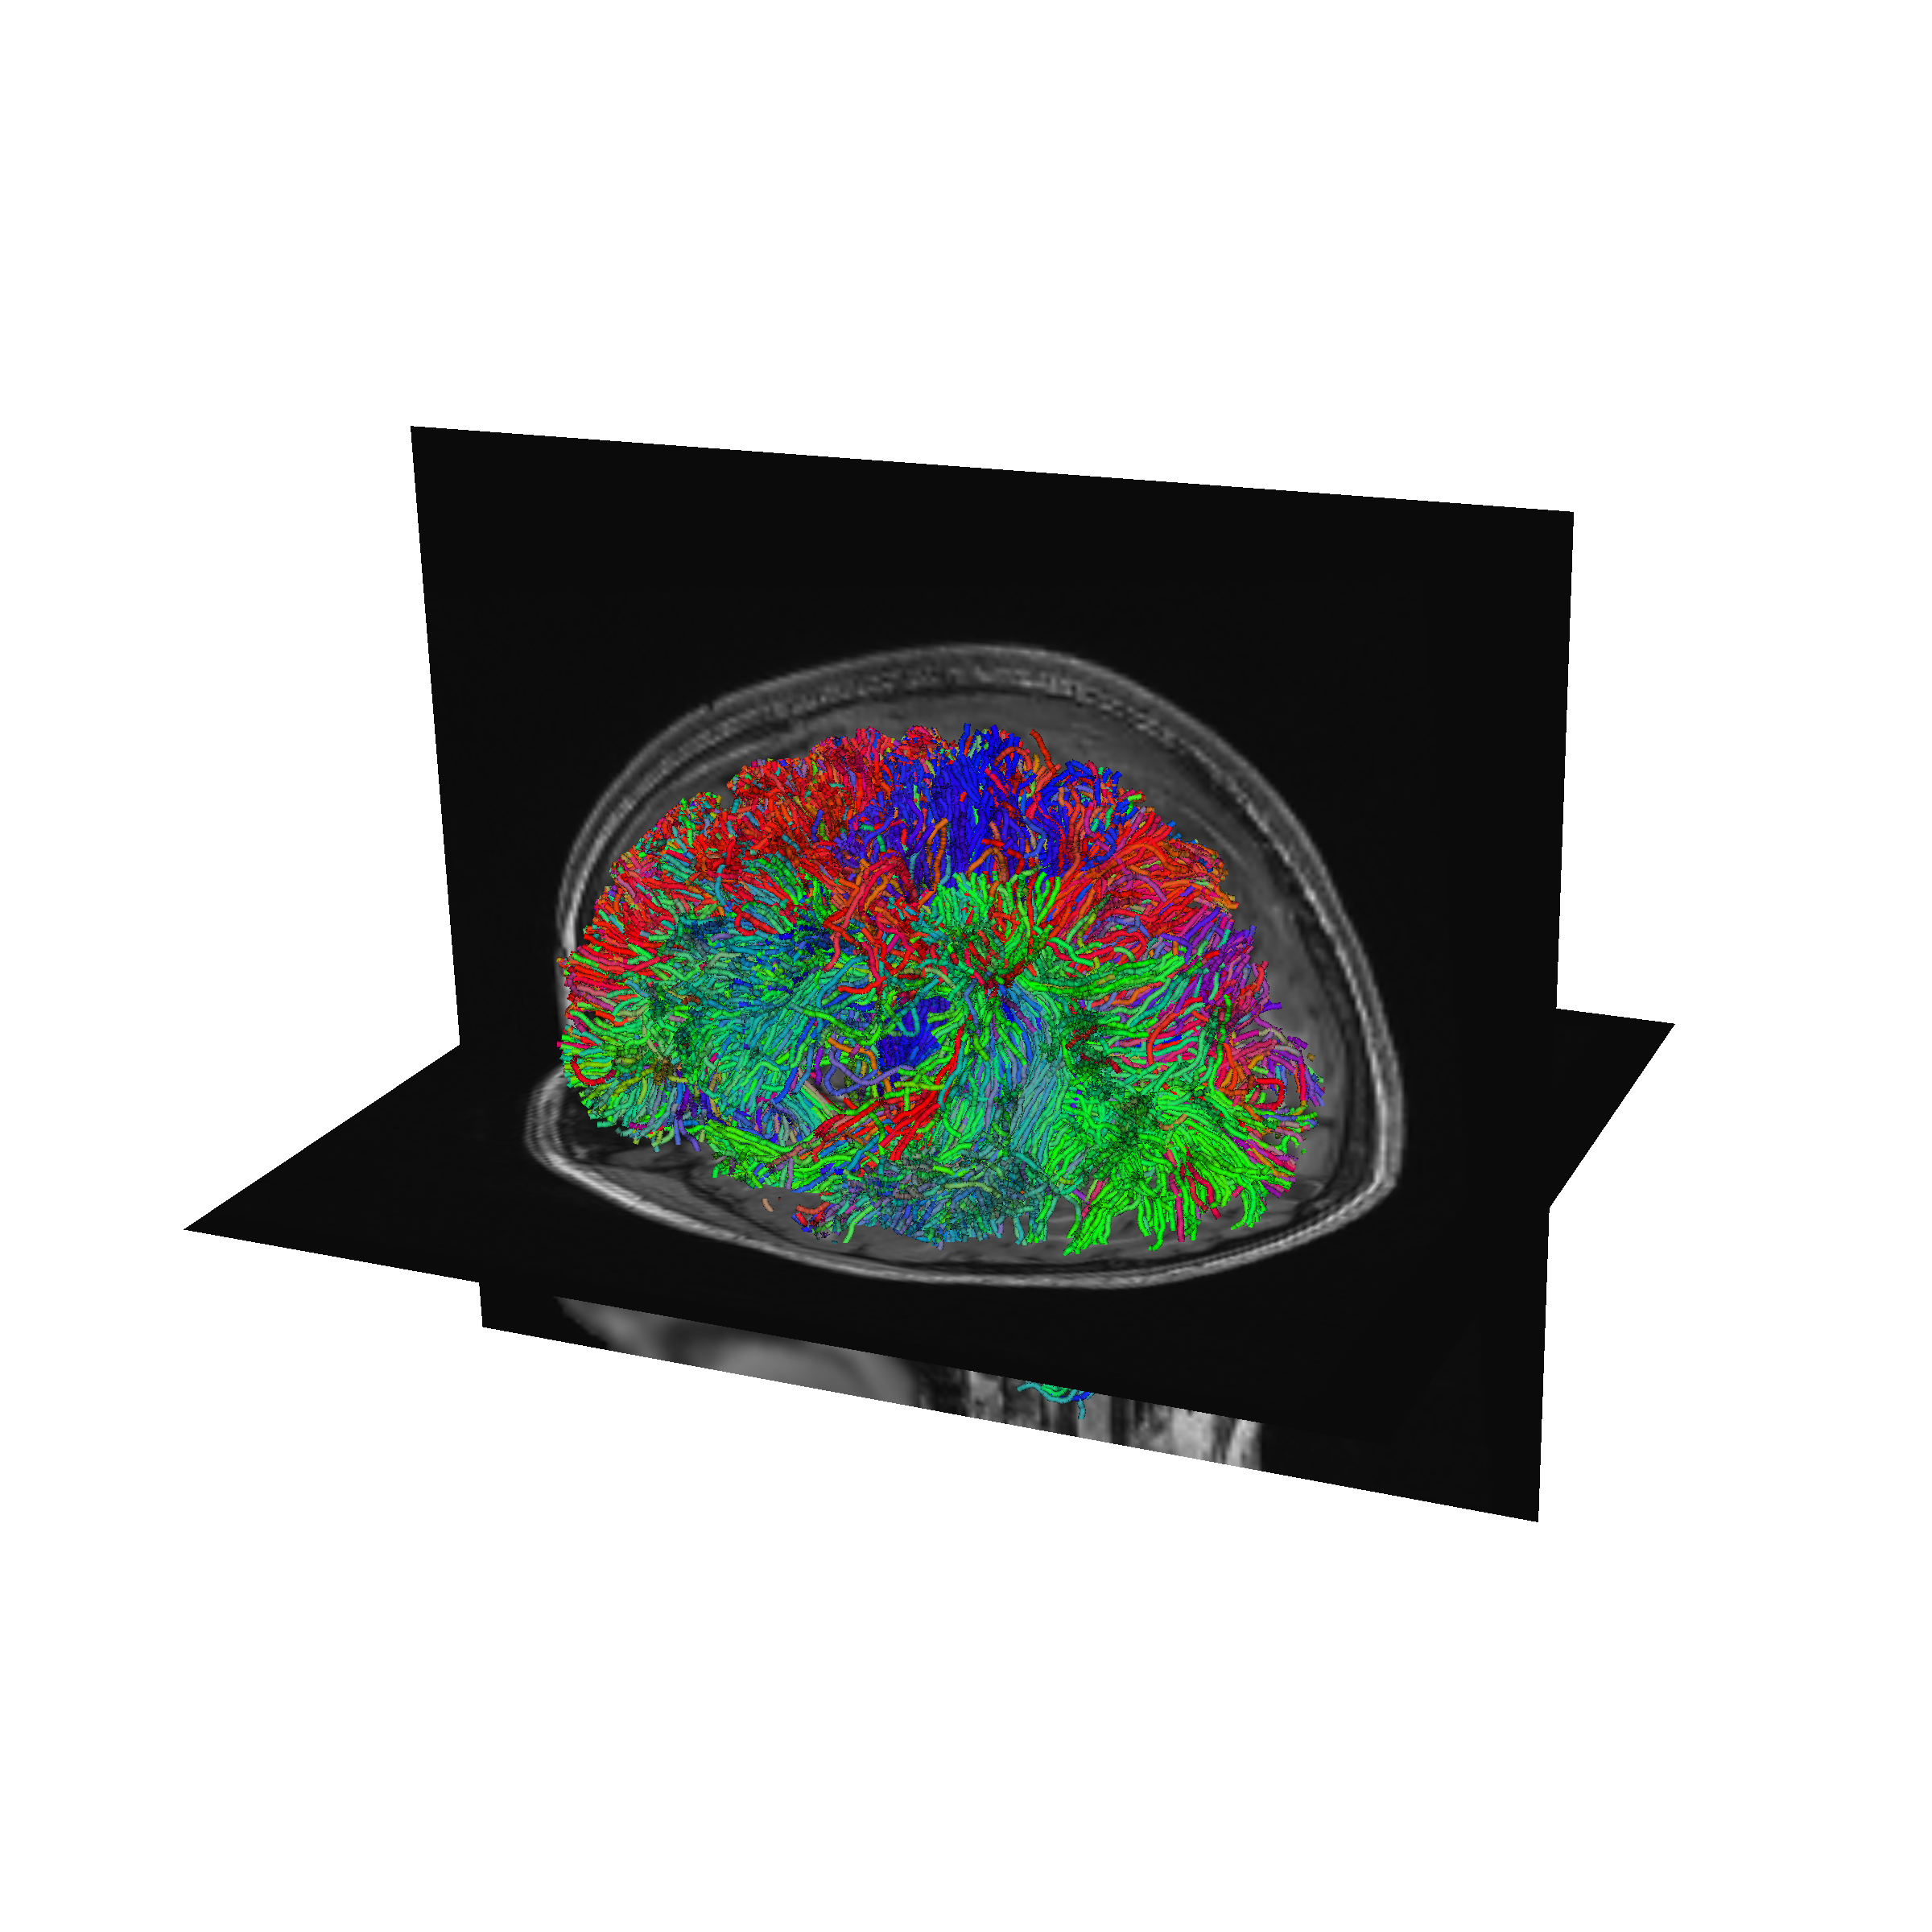
\includegraphics[width=1.0\linewidth]{figures/whole_brain_trk}
        Whole brain tractography
    \end{Figure}
    \columnbreak
    \begin{Figure}
        \centering
        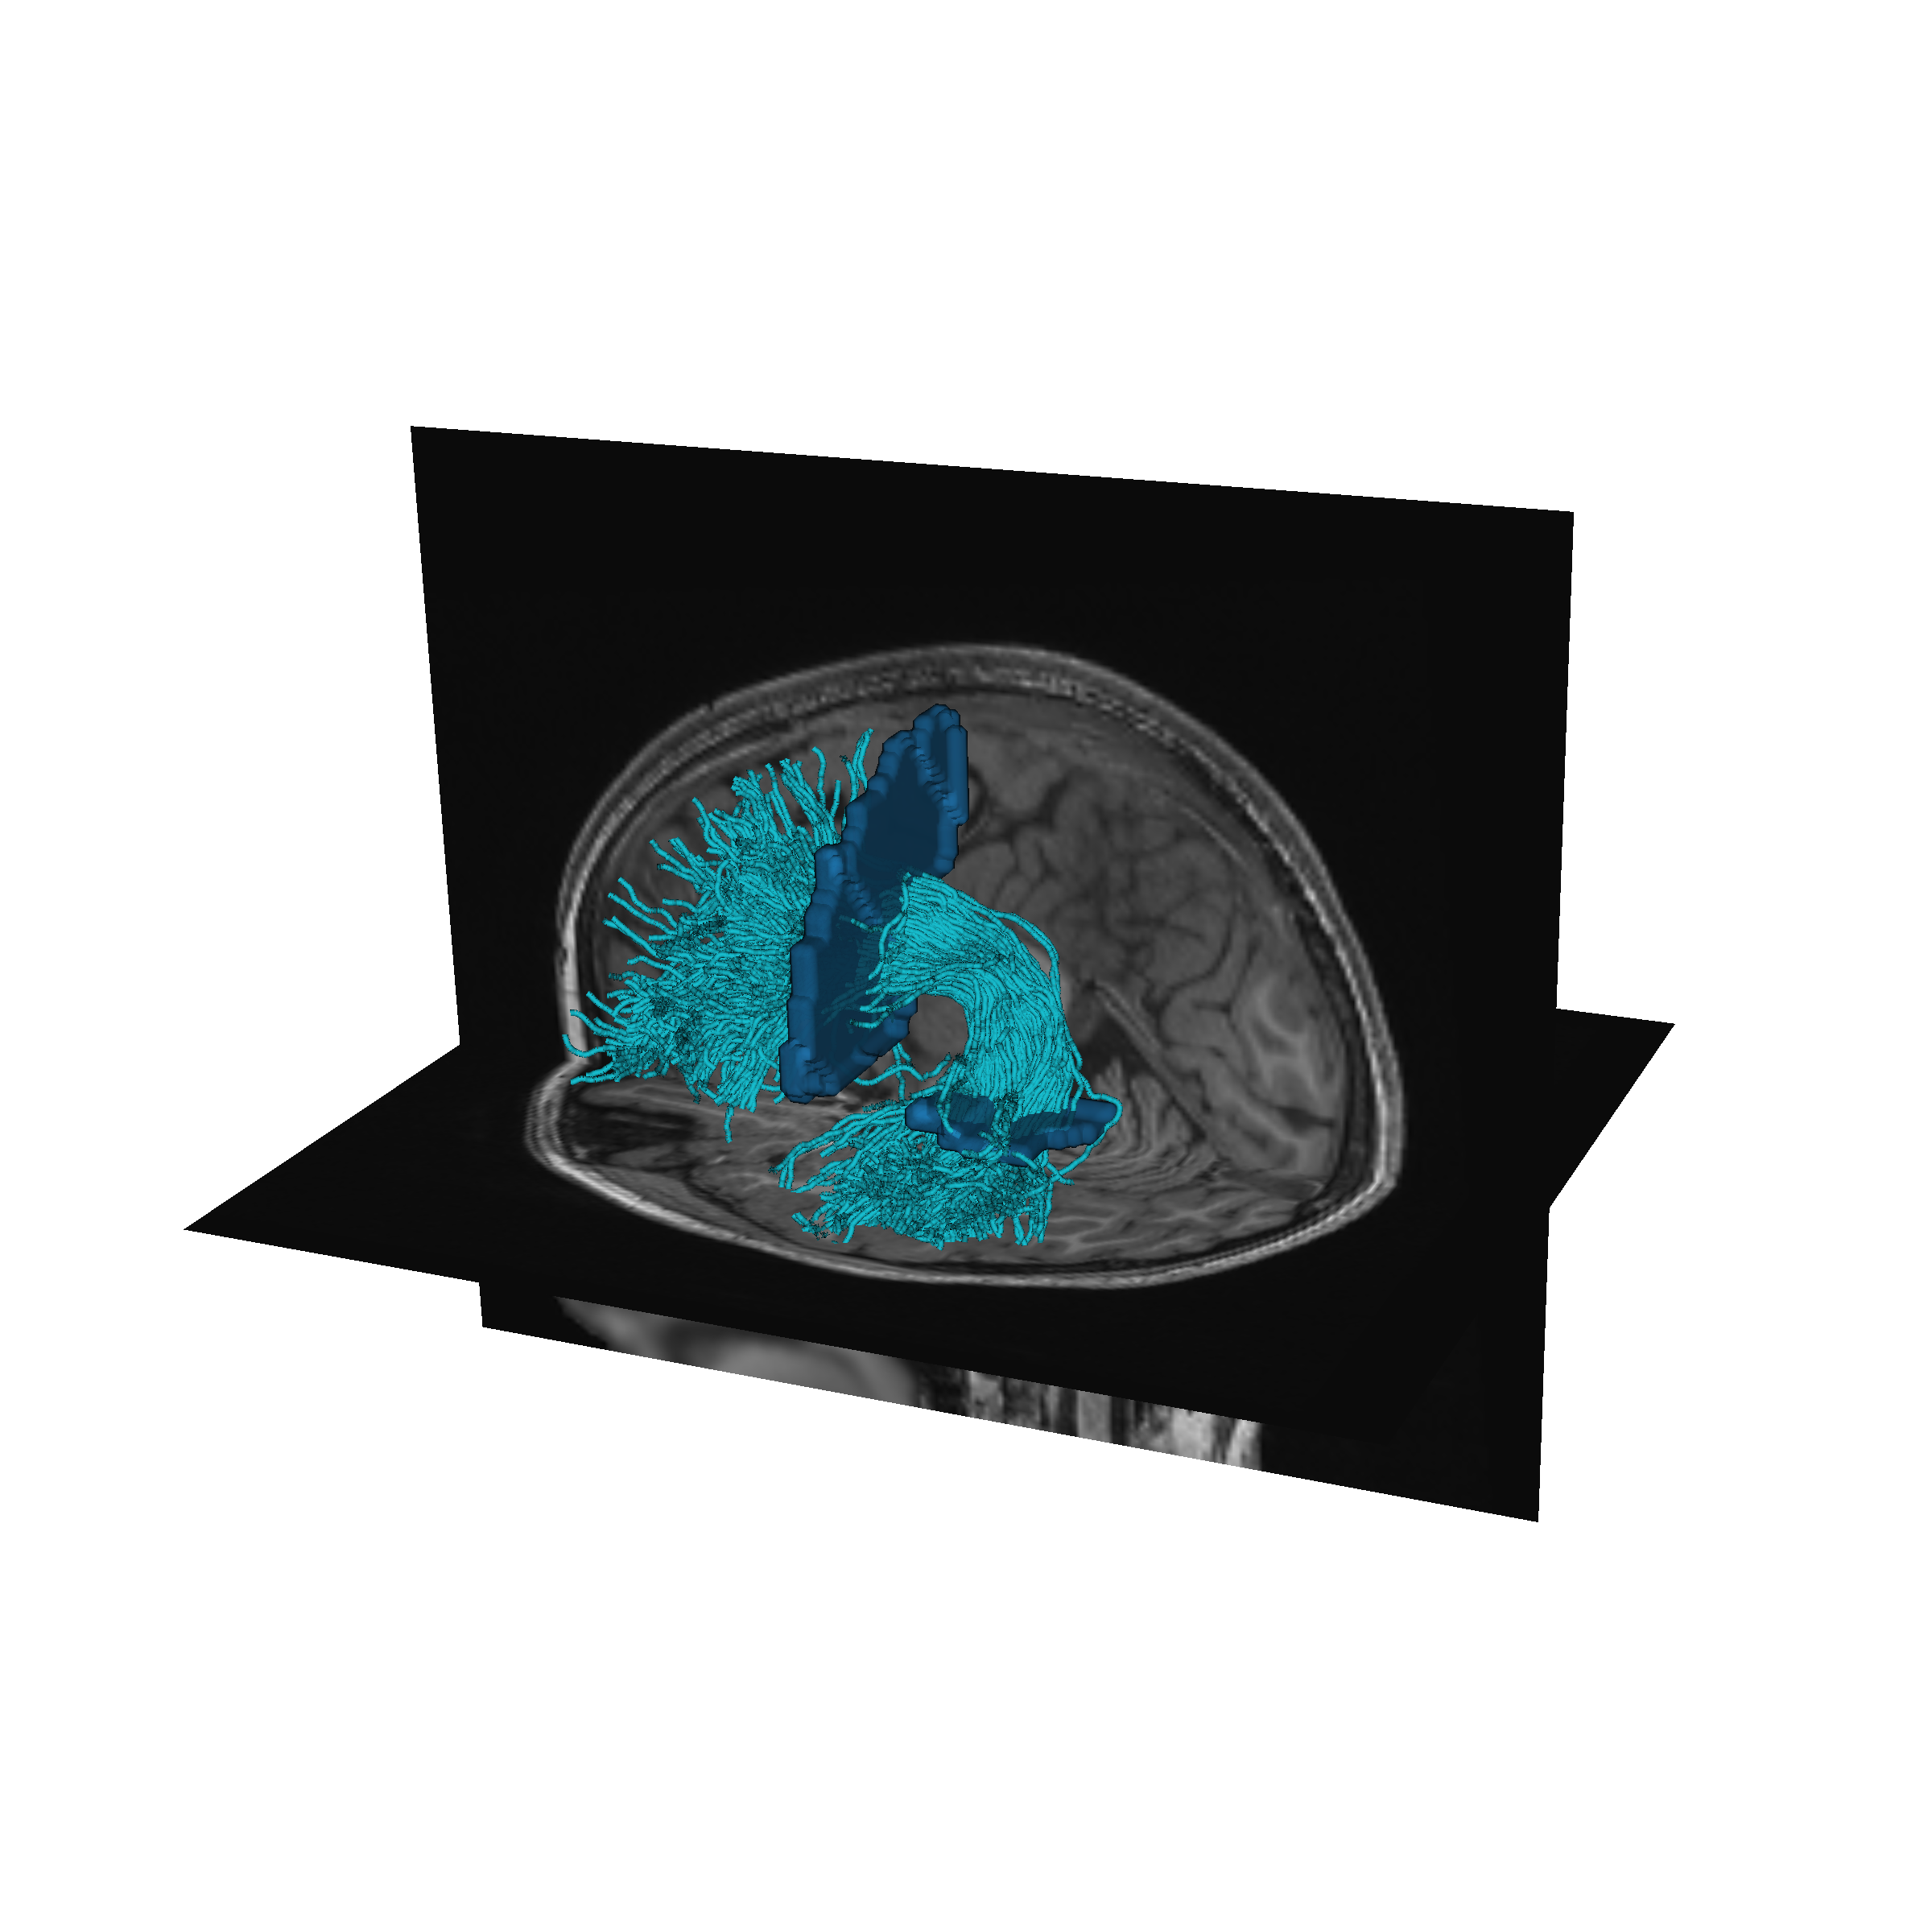
\includegraphics[width=1.0\linewidth]{figures/arc_trk}
        Selecting a bundle with ROIs
    \end{Figure}

    \columnbreak
    \begin{Figure}
        \centering
        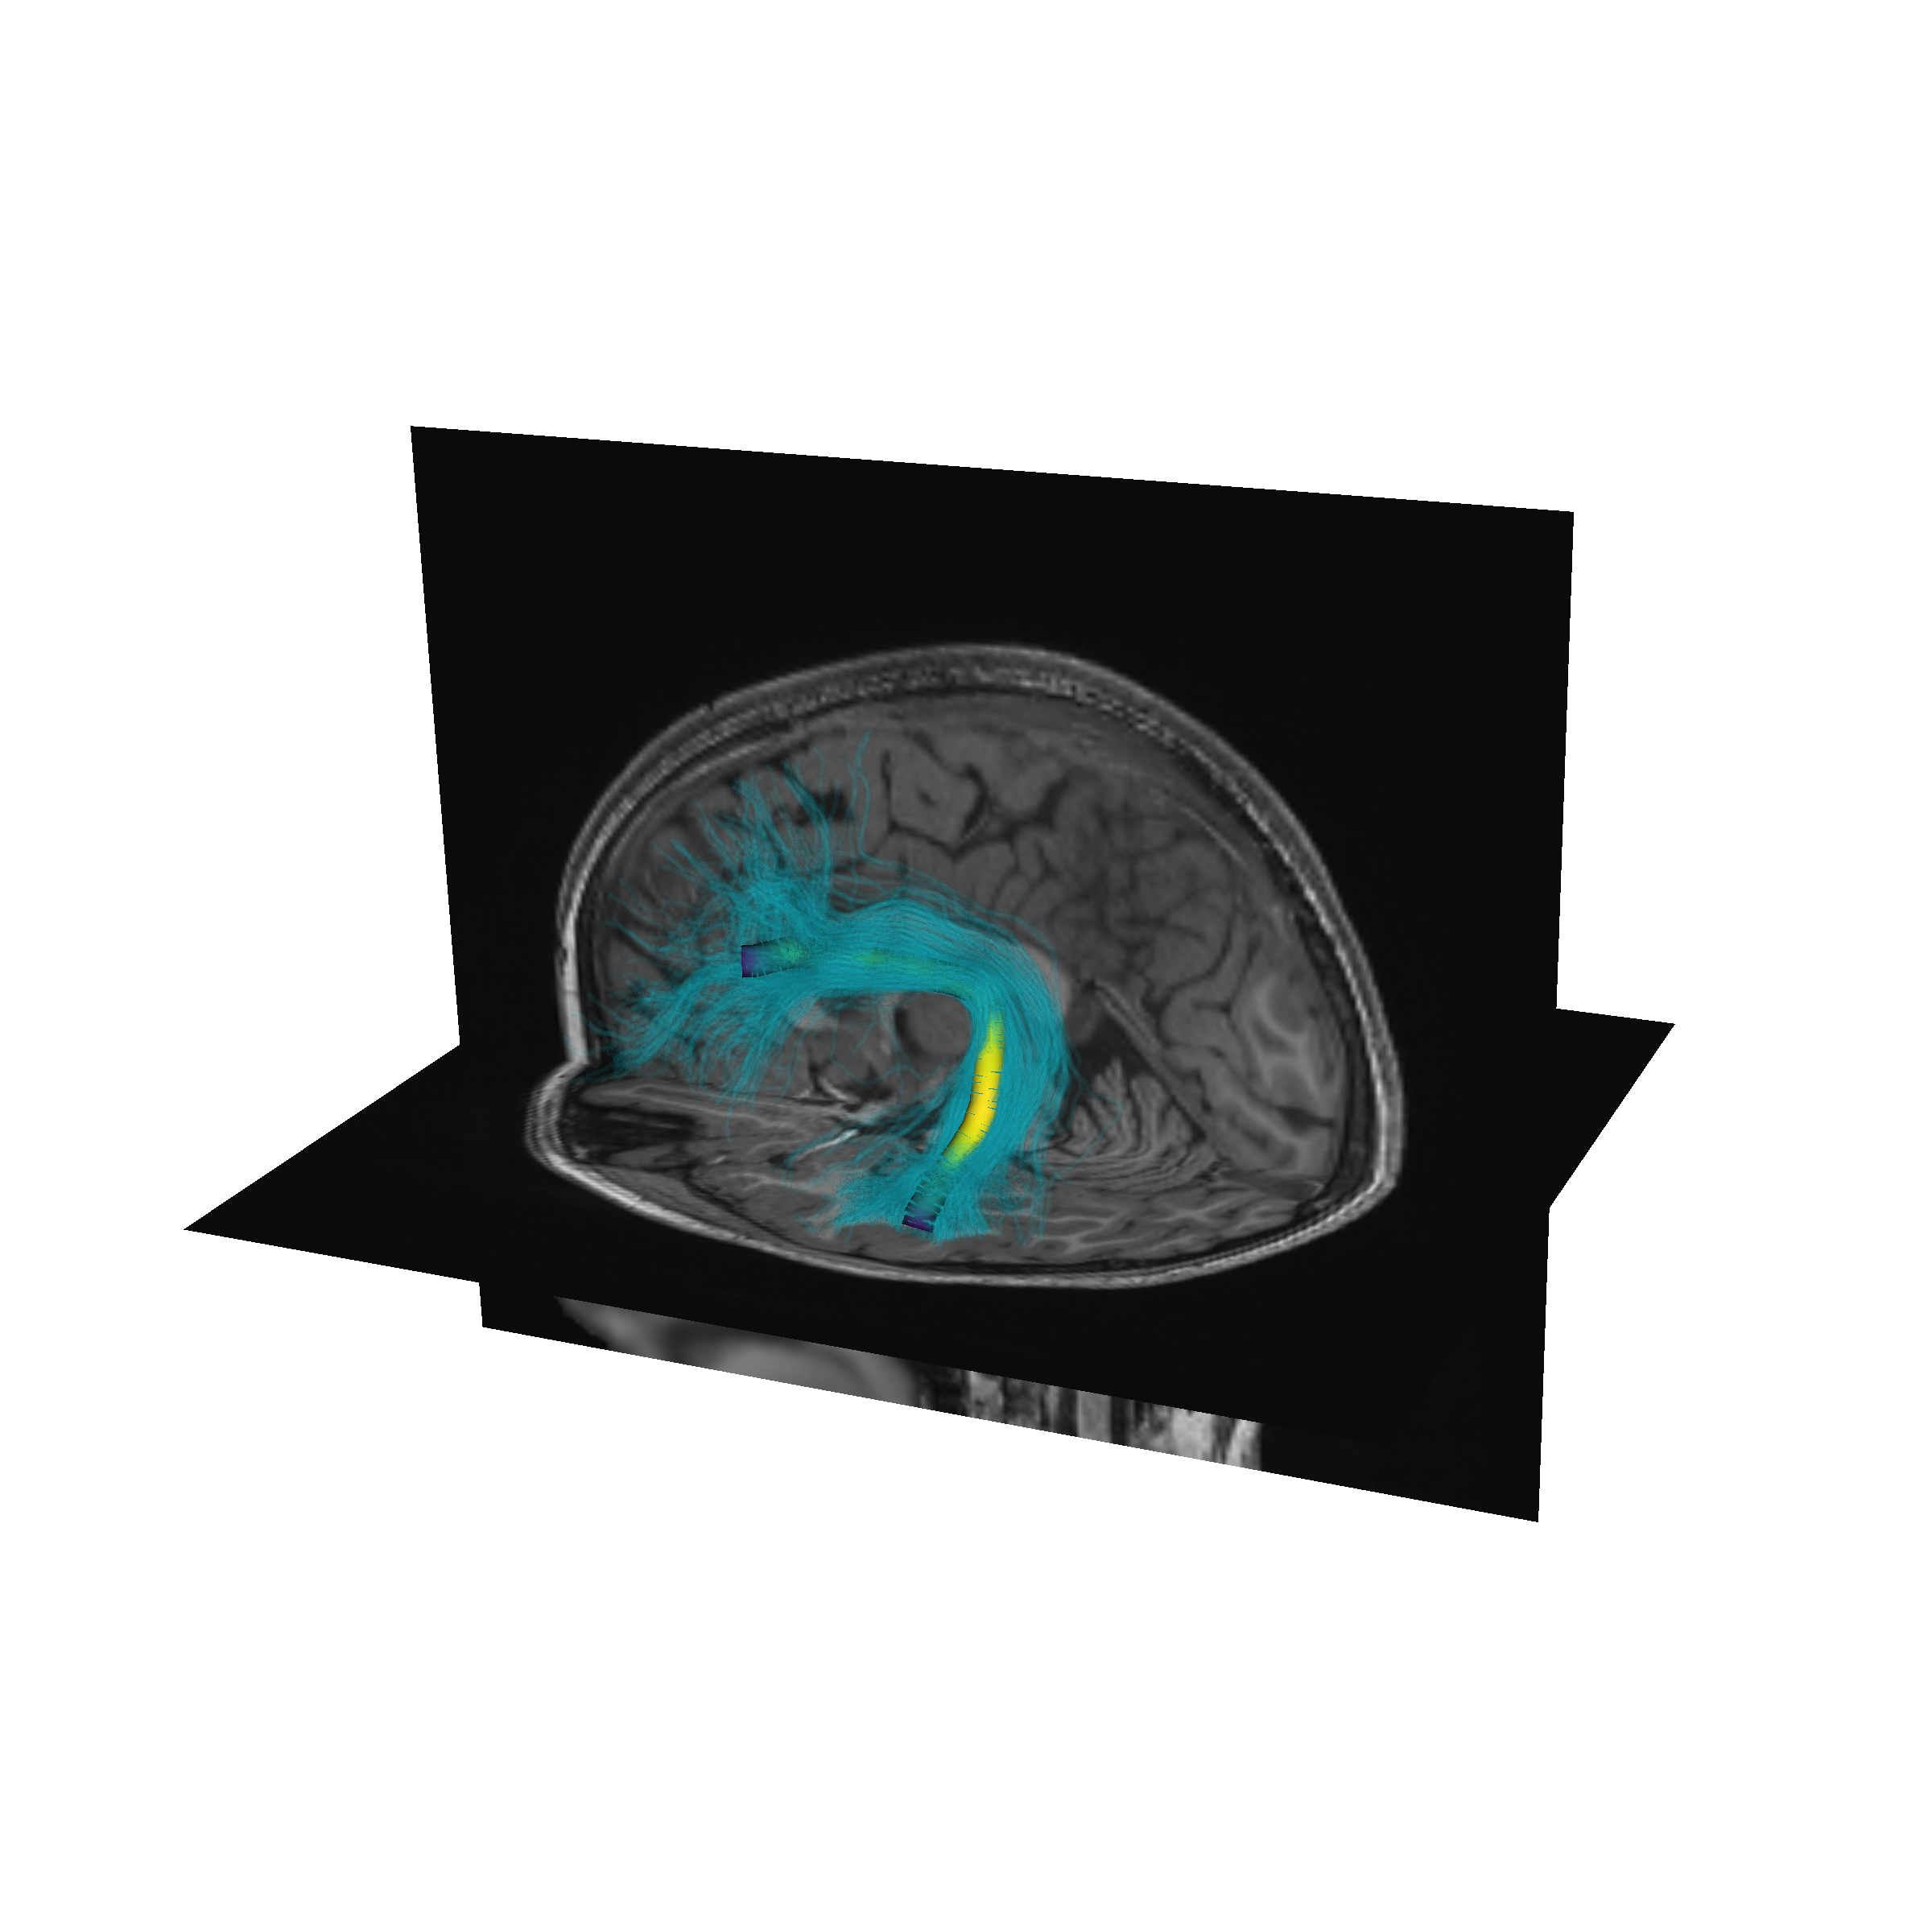
\includegraphics[width=1.0\linewidth]{figures/arc_profile_trk}
        Extracting values along the length of the tract
    \end{Figure}
    \columnbreak
    \begin{Figure}
        \vspace{1.0cm}
        \centering
        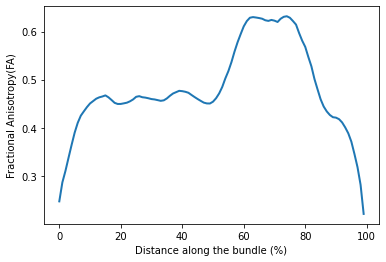
\includegraphics[width=1.0\linewidth]{figures/tract_profile}
        Tract profile
    \end{Figure}

    \vspace{2em}
\end{multicols}


\vspace{0.5em}
\noindent\textbf{%
    \underline{Question}: %
    Does deep learning provide improvements in inferences from tractometry?%
}
\vspace{0.5em}}

\headerbox{Methods}{name=methods, column=0, below=introduction, span=2}{
\begin{itemize}[nosep, leftmargin=*]
\end{itemize}

\begin{multicols}{3}
    \textbf{A}
    \begin{Figure}
        \centering
        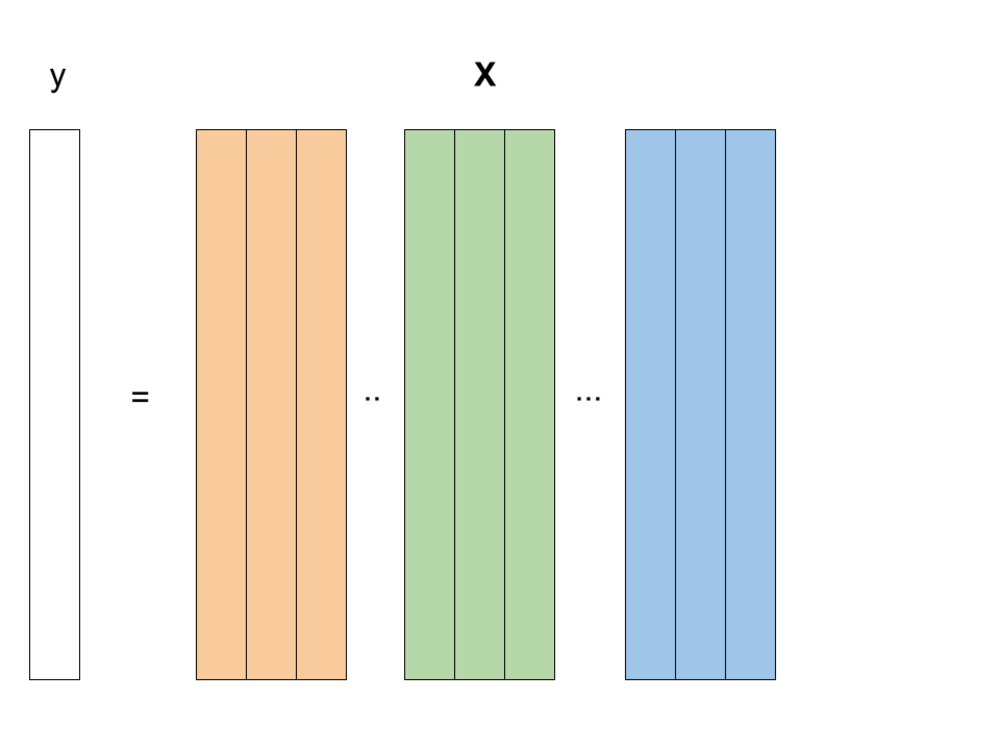
\includegraphics[height=3.5cm]{figures/linear-model.pdf}
    \end{Figure}
    \columnbreak
    \textbf{B}
    \begin{Figure}
        \centering
        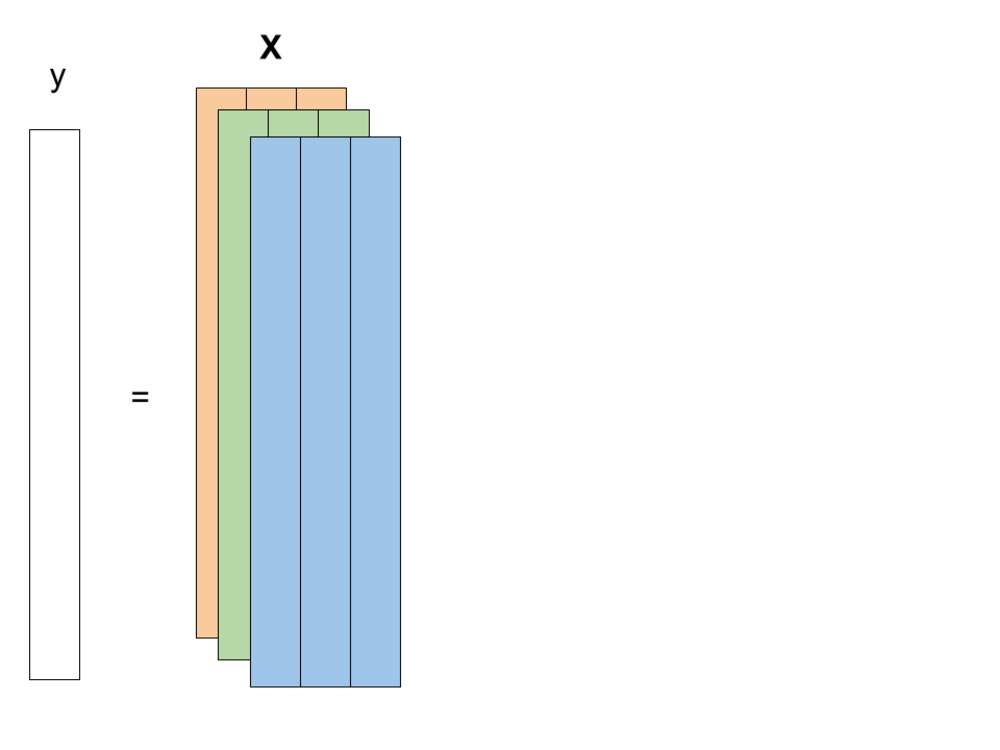
\includegraphics[height=4.5cm]{figures/linear-to-convnet.pdf}
    \end{Figure}
    \columnbreak
    \textbf{C}
    \begin{Figure}
        \centering
        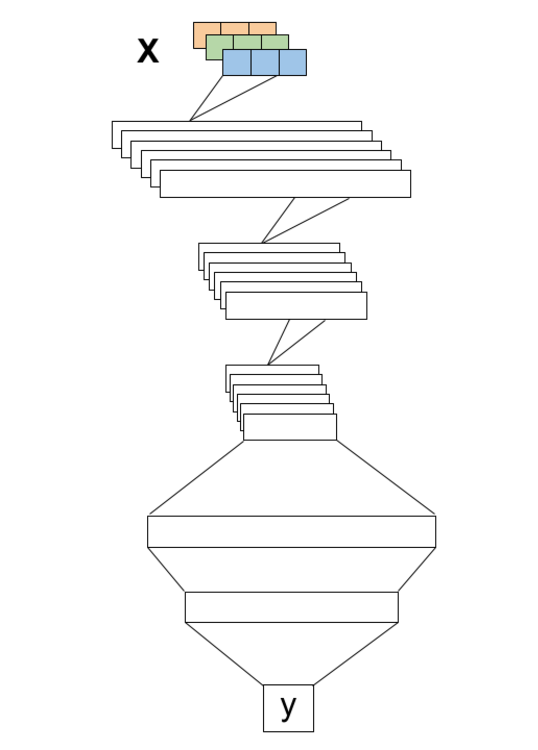
\includegraphics[height=4.5cm]{figures/convnet-schematic.pdf}
    \end{Figure}
\end{multicols}

\begin{itemize}[nosep, leftmargin=*]

\item (\textbf{A}) In a linear tractometry model, $\textbf{y} = \beta X$. (\textbf{B}) To move towards a convolutional neural networks, we stack the data from different tracts and metrics (FA, MD, MK) as different measurement ``channels'' . (\textbf{C}) Training samples are then passed to a network (here as schematic)

\item We used the 1817 subjects from HBN POD2 that had passing QC scores and age
information.

\item A variety of convolutional neural networks were implemented in \texttt{AFQ-Insight} (\url{https://richiehalford.org/AFQ-Insight})

\item We trained the models in ``brain age'' prediction. To evaluate the models, we set aside a test set of 20\% of the subjects (363 subjects)

\item To compare model dependence on training set size, we trained with variable train set sizes (100, 175, 350, 700, 1000, 1453 subjects) and different augmentation levels

\item We compared to a state-of-the-art linear model: PCR Lasso \cite{richford2021sgl}

\item Model performance was quantified as the coefficient of determination, $R^2$, in predicting the age of the test set subjects.

\item $R^2$ was modeled as: $\alpha - (\alpha - \beta) e^{-\frac{x - x_{min}}{\kappa}}$, where $x$ is the number of training samples, $\alpha$ is $R^2$ at the maximal number of training samples, $\beta$ is $R^2$ at the smallest number of training samples ($x_{min}$) and $\kappa$ is a free parameter that denotes that number of training samples required to achieve $R^2$ that is 67\% of the difference between $\beta$ and $\alpha$.

\end{itemize}
}

%----------------------------------------------------------------------------
%	RESULTS 1
%----------------------------------------------------------------------------

\headerbox{Results}{name=results, column=2, span=4, row=0}{

At each augmentation level, performance improves with training set size:

\begin{multicols}{4}
    \begin{Figure}
        \centering
        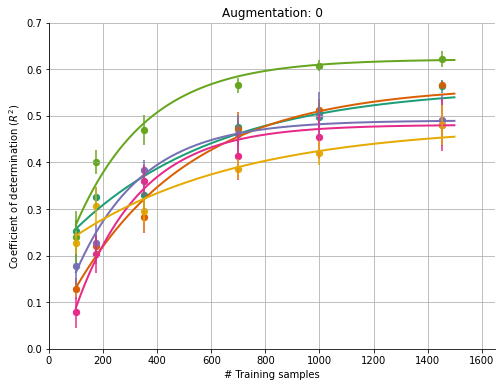
\includegraphics[width=1.0\linewidth]{figures/curves_aug_0}
    \end{Figure}
    \columnbreak

    \begin{Figure}
        \centering
        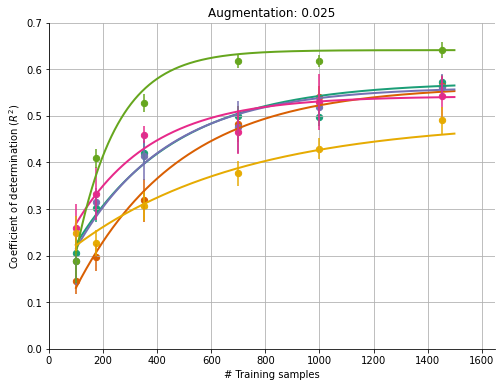
\includegraphics[width=1.0\linewidth]{figures/curves_aug_40}
    \end{Figure}
    \columnbreak

    \begin{Figure}
        \centering
        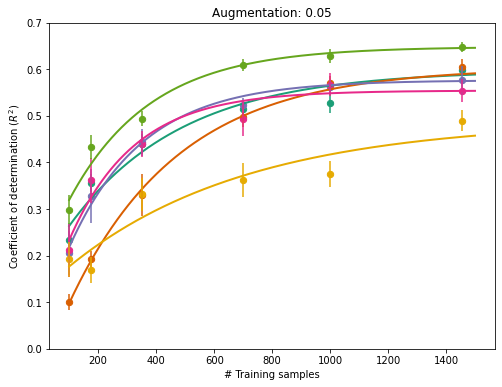
\includegraphics[width=1.0\linewidth]{figures/curves_aug_20}
    \end{Figure}

    \columnbreak

    \begin{minipage}[c]{0.3\linewidth}
    \begin{Figure}
    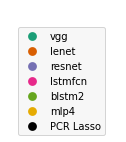
\includegraphics[height=2.5cm]{figures/legend}
    \end{Figure}
    \end{minipage}
    \begin{minipage}[c]{0.6\linewidth}
    \begin{framed}
        \small
        \textbf{Model categories} \\
        \textbf{Convlutional neural networks}: lenet, vgg, resnet \\
        \textbf{Fully connected neural network}: mlp4 \\
        \textbf{Recurrent neural networks}: blstm2, lstmfcn \\
        \textbf{Baseline linear model}: lassopcr
    \end{framed}
    \end{minipage}
\end{multicols}
\\
\begin{multicols}{4}
    \begin{Figure}
        \centering
        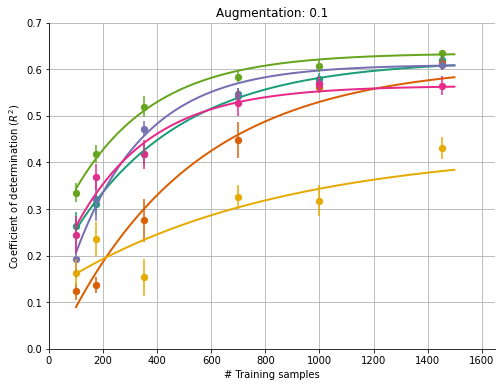
\includegraphics[width=1.0\linewidth]{figures/curves_aug_10}
    \end{Figure}

    \columnbreak
    \begin{Figure}
        \centering
        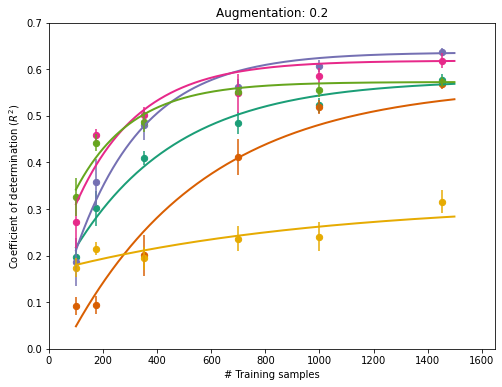
\includegraphics[width=1.0\linewidth]{figures/curves_aug_5}
    \end{Figure}

    \columnbreak
    \begin{Figure}
        \centering
        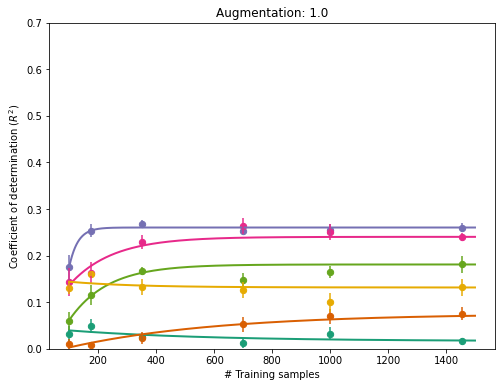
\includegraphics[width=1.0\linewidth]{figures/curves_aug_1}
    \end{Figure}

    \columnbreak
    \begin{Figure}
        \centering
        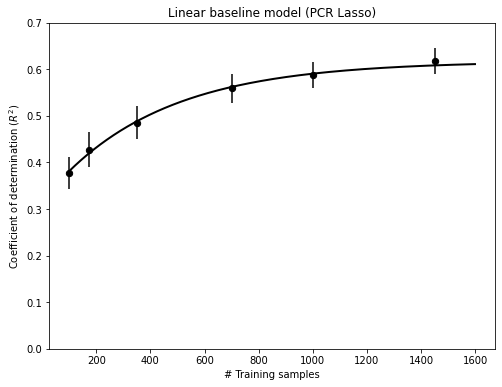
\includegraphics[width=1.0\linewidth]{figures/curves_pcrlasso}
    \end{Figure}
    \columnbreak

\end{multicols}

The models' performance at each augmentation level is summarized through three parameters that quantify the maximal ($\alpha$) and minimal ($\beta$) performance levels, and the convergence of performance with training set size ($\kappa$):

\begin{multicols}{3}
    \begin{Figure}
        \centering
        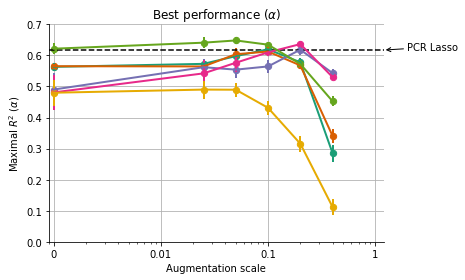
\includegraphics[width=0.9\linewidth]{figures/max_acc}
    \end{Figure}
    \columnbreak
    \begin{Figure}
        \centering
        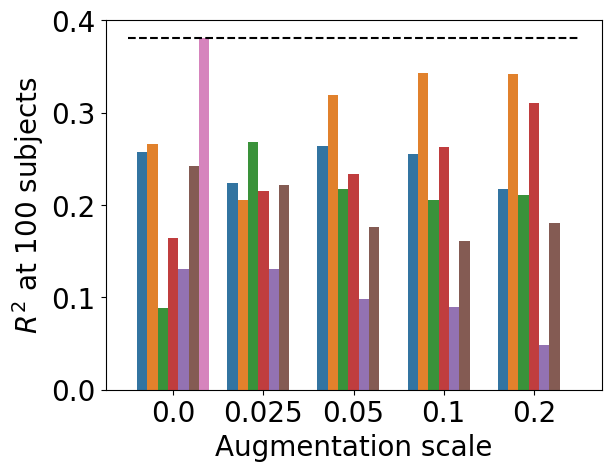
\includegraphics[width=0.9\linewidth]{figures/min_acc}
    \end{Figure}

    \columnbreak
    \begin{Figure}
        \centering
        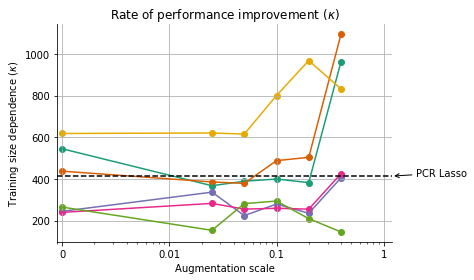
\includegraphics[width=0.9\linewidth]{figures/num_subjects}
    \end{Figure}

    \vspace{2em}
\end{multicols}

}

%----------------------------------------------------------------------------
%	CONCLUSION
%----------------------------------------------------------------------------

\headerbox{Conclusion and future work}{name=conclusion, column=2, span=3, below=results}{
\begin{multicols}{2}
\begin{itemize}
\item Neural network models (NNs) improve accuracy of tractometry analysis
\item NNs are very data hungry
\item Recurrent neural networks seem to perform most accurately, with moderate augmentation levels required.

\columnbreak
\item Tuning and training these models is complicated and time-consuming
\item Differences between linear models and NN models can be \emph{qualitative}, where NN models find differences not detected by linear models  (see poster \# 387.05 on Monday afternoon)

\end{itemize}
\end{multicols}


}

%----------------------------------------------------------------------------
%   REFERENCES
%----------------------------------------------------------------------------

\headerbox{References}{name=references, column=2, span=3, below=conclusion,above=bottom}{

\begin{multicols}{2}
\smaller \smaller % Reduce the font size in this block
\renewcommand{\section}[2]{\vskip 0.05em} % Get rid of the default "References" section title
\nocite{*} % Insert publications even if they are not cited in the poster

% \printbibliography
\bibliographystyle{unsrt}
\bibliography{poster}
\end{multicols}
}

%----------------------------------------------------------------------------
%	ACKNOWLEDGMENTS
%----------------------------------------------------------------------------

\headerbox{Acknowledgments}{name=acknowledgments, column=5, span=1, below=results,above=bottom}{

Grant 1RF1MH121868\\
\vspace{0.00001cm}\\


\includegraphics[align=c, height=1.0cm]{logos/nimh-logo.png}\\
\vspace{0.1cm}\\

\includegraphics[align=c, height=1.0cm]{logos/awslogo}\\
\vspace{0.1cm}\\

\includegraphics[align=c, height=1.0cm]{logos/azure}\\
\vspace{0.1cm}\\

\includegraphics[align=c, height=1.0cm]{logos/eSciencelogo.png}

}

\end{poster}

\end{document}
